\documentclass[11pt,letterpaper]{article}
\usepackage[T1]{fontenc}
\usepackage{lmodern,microtype}
\usepackage[margin=0.78in,headheight=15pt,headsep=15pt]{geometry}
\usepackage{mathtools,amssymb}
\usepackage{xcolor,booktabs,array,tikz}
\usepackage[most]{tcolorbox}
\usepackage{enumitem,fancyhdr,needspace,hyperref}
\definecolor{ink}{HTML}{162332}
\definecolor{navy}{HTML}{17324D}
\definecolor{teal}{HTML}{167D82}
\definecolor{mist}{HTML}{EDF5F4}
\definecolor{muted}{HTML}{5D6B78}
\color{ink}
\hypersetup{colorlinks=true,linkcolor=teal,urlcolor=teal,pdfauthor={Igor Rivin}}
\setlength{\parindent}{0pt}
\setlength{\parskip}{4pt}
\setlength{\abovedisplayskip}{7pt}
\setlength{\belowdisplayskip}{7pt}
\setlist[enumerate]{label=(\alph*),leftmargin=1.8em,itemsep=3pt,topsep=4pt}
\newcommand{\Z}{\mathbb Z}
\newcommand{\F}{\mathbb F}
\newcommand{\one}{\mathbf{1}}
\newcommand{\id}{\operatorname{id}}
\newcommand{\pts}[1]{\hfill\textcolor{muted}{\small[#1 points]}}
\newcommand{\partpts}[1]{\unskip\nobreak\hspace{.4em}\textcolor{muted}{\small(#1)}}
\newcommand{\edition}{\ifsolutions Instructor solutions\else Student handout\fi}
\newcounter{problem}
\newcommand{\problem}[2]{\par\addvspace{11pt}\Needspace{6\baselineskip}%
  \stepcounter{problem}{\bfseries\color{navy}\theproblem.\ #1}\pts{#2}\par\nobreak}
\newcommand{\topic}[1]{\par\addvspace{9pt}\Needspace{10\baselineskip}%
  {\large\bfseries\color{teal}#1}\par\nobreak}
\newcommand{\studentbreak}{\ifsolutions\else\newpage\fi}
\newcommand{\challenge}[1]{\par\addvspace{12pt}\Needspace{7\baselineskip}%
  {\bfseries\color{teal}Optional challenge: #1}\pts{10 extra}\par\nobreak}
\pagestyle{fancy}
\fancyhf{}
\fancyhead[L]{\small\color{muted}\setname}
\fancyhead[R]{\small\color{muted}Patterns, Proofs, and Primes}
\fancyfoot[L]{\footnotesize\color{muted}\edition}
\fancyfoot[R]{\small\color{teal}\thepage}
\renewcommand{\headrulewidth}{0.3pt}
\NewDocumentEnvironment{solution}{+b}{\ifsolutions
  \begin{tcolorbox}[enhanced,breakable,colback=mist!45,colframe=teal!45,
    boxrule=.5pt,arc=1mm,left=3mm,right=3mm,top=2mm,bottom=2mm,
    before skip=7pt,after skip=7pt,title={Solution},
    title after break={Solution (continued)},colbacktitle=mist,
    coltitle=teal,fonttitle=\small\bfseries]
  \small #1
  \end{tcolorbox}\fi}{}
\newcommand{\handouttitle}[3]{%
  {\LARGE\bfseries\color{navy}\setname}\hfill{\small\color{teal}\edition}\\[4pt]
  {\large #1}\\[4pt]{\small\color{muted}#2}\par
  \medskip\textbf{Preparation.} #3\par
  \ifsolutions\else\medskip
  \textbf{Name:}\ \rule{.46\linewidth}{.4pt}\hfill
  \textbf{Due:}\ \rule{.20\linewidth}{.4pt}\par\fi}

\newcommand{\setname}{Problem Set 4}
\hypersetup{pdftitle={Number Theory Problem Set 4: Orders, Interpolation, and Fourier Inversion},
  pdfsubject={Optional enrichment: poset Mobius inversion and finite Fourier transforms}}
\begin{document}
\handouttitle{Orders, interpolation, and Fourier inversion}
{Optional enrichment \textbar\ 6 problems \textbar\ 80 points + 10 challenge points
\textbar\ Suggested time: 3--4 hours}
{Course packet Sections 5.10--5.11 and polynomial interpolation from Chapter 4.
Use $i^2=-1$ for complex arithmetic; no calculus or infinite Fourier series is needed.}

\textbf{Instructions.} Write on separate paper and use exact arithmetic.
You may use poset M\"obius inversion and polynomial CRT, except when a
problem asks you to establish the relevant formula. Problems 1--3 concern
order and counting; Problems 4--6 concern polynomial evaluation and its inverse.

\textbf{Conventions.} For a finite poset $P$, $\mu_P(x,x)=1$ and
$\mu_P(x,y)=-\sum_{x\le z<y}\mu_P(x,z)$ when $x<y$.
For a primitive $n$th root $\omega$, our Fourier convention is
\[
 y_j=\sum_{k=0}^{n-1}c_k\omega^{jk},\qquad
 c_k=\frac1n\sum_{j=0}^{n-1}y_j\omega^{-jk}.
\]
Over a finite field, $1/n$ means a multiplicative inverse in that field.

\ifsolutions
\textbf{Grading note.} This is an optional enrichment assignment; subpart
scores total 80, with 10 extra challenge points. Sections I and II can also
be assigned independently. Accept either recursive subtraction or an
explicit M\"obius formula where appropriate. Check the direction of the order,
the Fourier sign convention, and the factor $1/n$ in addition to arithmetic.
\fi

\topic{I. Recover exact counts from cumulative counts}

\problem{Four incomparable middle elements}{12}
Let $P=\{0,a,b,c,d,1\}$, with $0<x<1$ for each
$x\in\{a,b,c,d\}$ and no comparisons between distinct middle elements.
\begin{enumerate}
 \item Draw the Hasse diagram and list the intervals with exactly two
 elements. \partpts{3}
 \item Compute $\mu_P(0,x),\mu_P(x,1)$ for the middle elements and
 $\mu_P(0,1)$. \partpts{4}
 \item Suppose $G(y)=\sum_{x\le y}F(x)$ and
 \[
 \begin{array}{c|rrrrrr}
 y&0&a&b&c&d&1\\\hline
 G(y)&3&5&8&10&4&25
 \end{array}
 \]
 Recover all six values of $F$. Check $F(1)$ both by subtraction and
 by M\"obius inversion. \partpts{5}
\end{enumerate}
\begin{solution}
The two-element intervals are $[0,x]$ and $[x,1]$ for the four middle elements.
\begin{center}
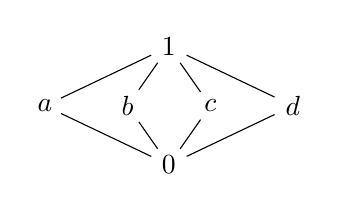
\begin{tikzpicture}[scale=.75,every node/.style={circle,fill=white,inner sep=2pt}]
 \node (lo) at (0,0) {$0$}; \node (hi) at (0,2) {$1$};
 \node (a) at (-2.1,1) {$a$}; \node (b) at (-.7,1) {$b$};
 \node (c) at (.7,1) {$c$}; \node (d) at (2.1,1) {$d$};
 \foreach \v in {a,b,c,d} {\draw (lo)--(\v)--(hi);}
\end{tikzpicture}
\end{center}
Each two-element interval has M\"obius value $-1$, so
$\mu_P(0,1)=-(1-4)=3$. Successive subtraction gives
\[
 (F(0),F(a),F(b),F(c),F(d),F(1))=(3,2,5,7,1,7).
\]
In particular $F(1)=25-(3+2+5+7+1)=7$. Inversion gives the same answer:
$F(1)=3G(0)-G(a)-G(b)-G(c)-G(d)+G(1)=9-27+25=7$.
\end{solution}

\problem{Membership patterns, including none}{14}
A universe $U$ has $50$ elements, and three subsets satisfy
\[
 |A|=24,\quad |B|=22,\quad |C|=18,\qquad
 |A\cap B|=10,\quad |A\cap C|=8,\quad |B\cap C|=6,\qquad
 |A\cap B\cap C|=3.
\]
\begin{enumerate}
 \item For $T\subseteq\{A,B,C\}$, let $F(T)$ count elements belonging
 to exactly the sets in $T$. Let $G(S)$ count elements in every set in $S$,
 with $G(\varnothing)=50$. Explain why
 $G(S)=\sum_{T\supseteq S}F(T)$ is an \emph{upper} sum on the subset poset.
 \partpts{4}
 \item Use upper-sum M\"obius inversion to recover all eight exact
 membership counts, including $F(\varnothing)$. State the formula used.
 \partpts{8}
 \item Compute $|A\cup B\cup C|$. Check that your eight counts are
 nonnegative and sum to $50$. \partpts{2}
\end{enumerate}
\begin{solution}
An element counted by $G(S)$ has an exact membership set $T$ containing $S$.
Since $\mu(S,T)=(-1)^{|T|-|S|}$ on the subset poset, upper inversion gives
\[
 F(S)=\sum_{T\supseteq S}(-1)^{|T|-|S|}G(T).
\]
For example, $F(\{A\})=24-10-8+3=9$, while
$F(\varnothing)=50-24-22-18+10+8+6-3=7$.
The complete table is
\[
\begin{array}{c|rrrrrrrr}
 S&\varnothing&A&B&C&AB&AC&BC&ABC\\\hline
 F(S)&7&9&9&7&7&5&3&3
\end{array}
\]
where $AB$ abbreviates $\{A,B\}$, and similarly for the other labels.
All entries are nonnegative and sum to $50$.
The union has $50-7=43$ elements, also $24+22+18-10-8-6+3$.
\end{solution}

\studentbreak
\problem{Why a partition coefficient can be six}{14}
Let $\Pi_4$ be the partitions of $\{1,2,3,4\}$, ordered by refinement.
Write $\hat0=1|2|3|4$ and $\hat1=1234$.
Partitions have block-size types $1+1+1+1$, $2+1+1$, $2+2$, $3+1$, or $4$.
\begin{enumerate}
 \item Count the partitions of each type. \partpts{4}
 \item Compute $\mu_{\Pi_4}(\hat0,\pi)$ for each type, ending with
 $\mu_{\Pi_4}(\hat0,\hat1)$ by the recurrence.
 \emph{Hint:} for type $2+2$, the interval is a product of two
 two-element chains; for type $3+1$, it is $\Pi_3$. \partpts{6}
 \item There are $a$ colors. Let $F(\rho)$ count colorings of four labeled
 positions whose equality partition is exactly $\rho$, and let $G(\pi)$
 count colorings constant on every block of $\pi$. Explain why
 $G(\pi)=a^{|\pi|}=\sum_{\rho\ge\pi}F(\rho)$, where $|\pi|$ counts blocks.
 Invert to count colorings with all four colors distinct. Give the result
 for $a=5$ and compare with direct counting. \partpts{4}
\end{enumerate}
\begin{solution}
The counts are obtained by choosing a pair, choosing an unordered pairing,
or choosing a triple, as applicable:
\[
\begin{array}{c|rrrrr}
 \text{type}&1+1+1+1&2+1+1&2+2&3+1&4\\\hline
 \text{number}&1&6&3&4&1\\
 \mu(\hat0,\pi)&1&-1&1&2&-6
\end{array}
\]
A two-element chain contributes $-1$, so a product of two contributes $1$.
For $\Pi_3$, the top coefficient is $-(1-3)=2$. Finally the proper elements
below $\hat1$ contribute $1-6+3+8=6$, so its coefficient is $-6$.

A coloring constant on blocks of $\pi$ may give the same color to different
blocks; its equality partition is therefore a coarsening $\rho\ge\pi$.
Upper inversion gives
\[
 F(\hat0)=\sum_{\pi\in\Pi_4}\mu(\hat0,\pi)a^{|\pi|}
 =a^4-6a^3+11a^2-6a=a(a-1)(a-2)(a-3).
\]
For $a=5$ this is $120$. Directly, the four labeled positions have
$a,a-1,a-2,a-3$ successive color choices.
\end{solution}

\topic{II. Recover coefficients from values}

\problem{Lagrange selectors become Fourier inversion}{12}
Let $n\ge2$ and let $\omega\in\mathbb C$ have order exactly $n$.
\begin{enumerate}
 \item Use a finite geometric sum to show, for every integer $m$,
 \[
 \sum_{j=0}^{n-1}\omega^{jm}=
 \begin{cases}n,&n\mid m,\\0,&n\nmid m.\end{cases}
 \]
 Explain where primitivity of $\omega$ enters. \partpts{4}
 \item Define $\ell_j(X)=\frac1n\sum_{k=0}^{n-1}\omega^{-jk}X^k$.
 Show that $\ell_j(\omega^r)=1$ for $r=j$ and $0$ otherwise,
 for $0\le r,j<n$. Explain why this identifies the Lagrange basis.
 \partpts{4}
 \item If $f(X)=\sum_{k=0}^{n-1}c_kX^k$ and $y_j=f(\omega^j)$,
 expand $f=\sum_j y_j\ell_j$ to derive the inverse Fourier formula.
 Explain the role of the degree restriction. \partpts{4}
\end{enumerate}
\begin{solution}
Primitivity says $\omega^m=1$ exactly when $n\mid m$. In that case all
$n$ terms equal $1$; otherwise their sum is
$(1-(\omega^m)^n)/(1-\omega^m)=0$.
Thus $\ell_j(\omega^r)=n^{-1}\sum_k\omega^{k(r-j)}$ has the stated values.
These polynomials have degree less than $n$, so uniqueness of interpolation
at $n$ distinct points makes them the Lagrange selectors.
Expanding the interpolant gives
\[
 f(X)=\sum_{j=0}^{n-1}y_j\left(\frac1n\sum_{k=0}^{n-1}\omega^{-jk}X^k\right)
 =\sum_{k=0}^{n-1}\left(\frac1n\sum_{j=0}^{n-1}y_j\omega^{-jk}\right)X^k.
\]
Comparing coefficients proves the inverse. Without the degree restriction,
values determine only the remainder modulo $X^n-1$; for example,
$f$ and $f+(X^n-1)$ have identical values at all these roots.
\end{solution}

\studentbreak
\problem{The same four-point transform in two fields}{16}
Take $f(X)=2-X+3X^3$, with coefficient vector $(2,-1,0,3)$.
For each field below, compute the four evaluations and then recover
the coefficients using the inverse transform, showing each inverse sum.
\begin{enumerate}
 \item Over $\mathbb C$, use $\omega=i$ and list values in the order
 $1,i,-1,-i$. \partpts{8}
 \item Over $\F_{13}$, prove that $\omega=5$ has order $4$.
 List values in the order $1,5,12,8$. Find both $\omega^{-1}$ and
 $4^{-1}$ before applying the inverse formula. Interpret the recovered
 coefficient of $X$. \partpts{8}
\end{enumerate}
\begin{solution}
Over $\mathbb C$, the value vector is $(4,2-4i,0,2+4i)$.
The four inverse sums give
\[
\begin{aligned}
 c_0&=\tfrac14[4+(2-4i)+0+(2+4i)]=2,\\
 c_1&=\tfrac14[4-i(2-4i)-0+i(2+4i)]=-1,\\
 c_2&=\tfrac14[4-(2-4i)+0-(2+4i)]=0,\\
 c_3&=\tfrac14[4+i(2-4i)-0-i(2+4i)]=3.
\end{aligned}
\]
\par\noindent\begin{minipage}{\linewidth}
In $\F_{13}$, $5^2=12=-1$ and $5^4=1$, so the order is $4$.
Its inverse is $8$, and $4^{-1}=10$.
The evaluations are $(4,8,0,9)$; for instance
$f(5)=2-5+3\cdot8=21\equiv8$. The inverse calculation is
\[
\begin{aligned}
 c_0&=10(4+8+0+9)=210\equiv2,\\
 c_1&=10(4+8\cdot8+12\cdot0+5\cdot9)=1130\equiv12,\\
 c_2&=10(4+12\cdot8+0+12\cdot9)=2080\equiv0,\\
 c_3&=10(4+5\cdot8+12\cdot0+8\cdot9)=1160\equiv3.
\end{aligned}
\]
All congruences are modulo $13$. The recovered vector is $(2,12,0,3)$,
which is $(2,-1,0,3)$ in this field.
\end{minipage}
\end{solution}

\problem{Why Fourier multiplication wraps around}{12}
Work over $\mathbb C$ with four evaluation points $1,i,-1,-i$.
Let $f(X)=1+2X+X^3$ and $g(X)=2+X^2$.
\begin{enumerate}
 \item Multiply ordinarily, then reduce modulo $X^4-1$ to find the
 unique remainder $h$ of degree less than $4$. \partpts{4}
 \item Compute the two value vectors, multiply them entry by entry,
 and invert to recover the coefficient vector of $h$. \partpts{4}
 \item Write the cyclic convolution formula for the coefficient of
 $X^r$ in $h$, using coefficient vectors $c=(1,2,0,1)$ and
 $d=(2,0,1,0)$. Explain why the $X^5$ term contributes to $X$,
 and how polynomial CRT justifies multiplication of values. \partpts{4}
\end{enumerate}
\begin{solution}
The ordinary product and its remainder are
\[
 fg=2+4X+X^2+4X^3+X^5,\qquad h=2+5X+X^2+4X^3.
\]
The value vectors are $(4,1+i,-2,1-i)$ and $(3,1,3,1)$;
their entrywise product is $y=(12,1+i,-6,1-i)$.
The four inverse numerators, before division by $4$, are
\[
\begin{aligned}
 &12+(1+i)-6+(1-i)=8,\\
 &12-i(1+i)+6+i(1-i)=20,\\
 &12-(1+i)-6-(1-i)=4,\\
 &12+i(1+i)+6-i(1-i)=16.
\end{aligned}
\]
Hence the coefficient vector is $(2,5,1,4)$, as above.
In general it is $(c*d)_r=\sum_{k=0}^3 c_kd_{(r-k)\bmod4}$.
Since $X^4=1$ in the quotient, $X^5=X$, so its coefficient wraps into
the coefficient of $X$. The four linear factors of $X^4-1$ are pairwise
coprime. Polynomial CRT identifies the quotient ring with four copies of
$\mathbb C$ via evaluation, and multiplication there is entry by entry.
\end{solution}

\ifsolutions\newpage\fi
\challenge{recover the ordinary product by adding zeros}
Use the same $f$ and $g$ as in Problem 6.
\begin{enumerate}
 \item What is the smallest transform length $N$ for which the
 remainder of $fg$ modulo $X^N-1$ must equal the ordinary product?
 Explain why length $8$ also works. \partpts{4}
 \item Work now over $\F_{17}$. Show that $2$ has order $8$ and find
 the inverse normalization factor $8^{-1}$. \partpts{3}
 \item Append zeros to make both coefficient vectors length $8$.
 Explain why evaluating at the powers of $2$, multiplying values,
 and inverting recovers the ordinary product over $\F_{17}$.
 Give the resulting length-$8$ coefficient vector; you need not compute
 the eight-point transforms explicitly. \partpts{3}
\end{enumerate}
\begin{solution}
The product has degree $5$, so $N=6$ is the smallest possible length;
any $N>5$, including $8$, prevents terms from wrapping.
In $\F_{17}$, $2^4=16=-1$ and $2^8=1$, so $2$ has order $8$.
The normalization is $8^{-1}=15$, since $8\cdot15=120\equiv1\pmod{17}$.
The padded vectors are $(1,2,0,1,0,0,0,0)$ and $(2,0,1,0,0,0,0,0)$.
CRT and Fourier inversion recover their product modulo $X^8-1$.
Its degree is only $5$, so it is already the ordinary product, with vector
$(2,4,1,4,0,1,0,0)$ in $\F_{17}^8$.
\end{solution}
\end{document}
